\documentclass{article}

\usepackage{titlesec}
\usepackage{titling}
\usepackage{graphicx}
\graphicspath{ {writeupimages/} }
\usepackage{float}
\usepackage{amsmath}

\titleformat{\section}
{\Large\bfseries}
{}
{0em}
{}[\titlerule]

\titleformat{\subsection}
{\large\bfseries}
{}
{0em}
{}

\titleformat{\subsubsection}
{\bfseries}
{}
{0em}
{}

\begin{document}

\title{Project: Kinematics Pick \& Place}
\author{Brett Gleason}

\maketitle

The rubric for this project can be found at the following URL: \\
https://review.udacity.com/\#!/rubrics/972/view \\
I will consider the rubric points individually and describe how I addressed each point in my implementation.  

\section{Writeup / README}

\subsection{1. Provide a Writeup / README that includes all the rubric points and how you addressed each one.  You can submit your writeup as markdown or pdf.}

You're reading it!

\section{Kinematic Analysis}
\subsection{1. Run the forward\_kinematics demo and evaluate the kr210.urdf.xacro file to perform kinematic analysis of Kuka KR210 robot and derive its DH parameters.}

Using the model of the Kuka KR210 robotic arm in the forward kinematics demo as well as the description of the joints within the URDF file, a schematic diagram of the robot can be drawn.

\begin{figure}[H]
    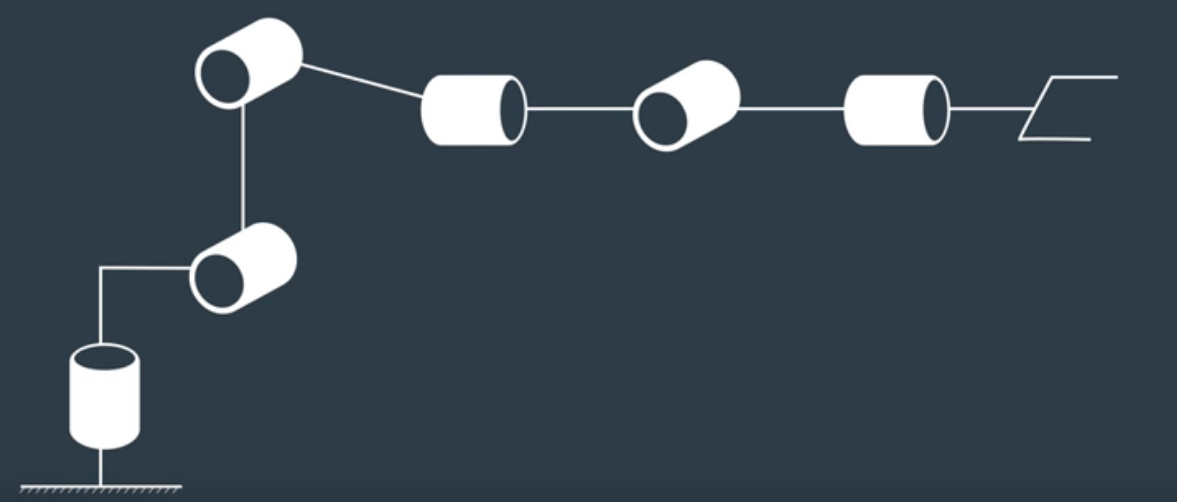
\includegraphics[width=\linewidth]{KR210scheme.png}
    \caption{Basic schematic as shown in project lesson 10}
    \label{fig:scheme}
\end{figure}

Next the joints are labeled from 1 to n and the links are labeled from 0 to n.

\begin{figure}[H]
    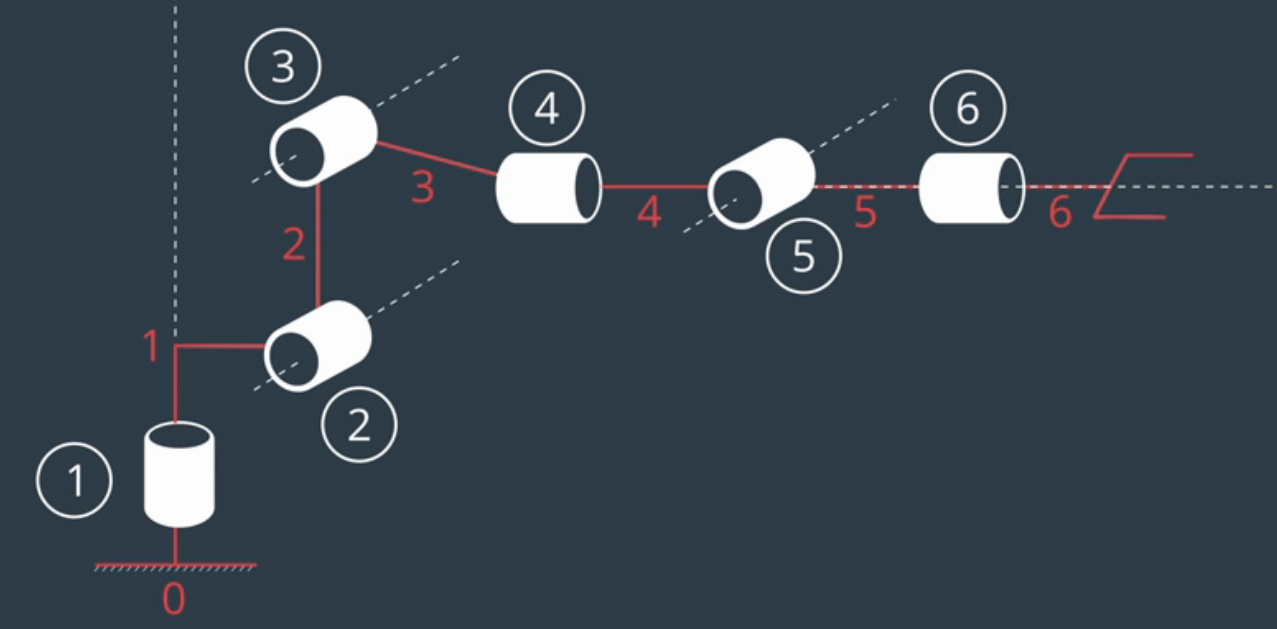
\includegraphics[width=\linewidth]{KR210JL.png}
    \caption{Schematic showing joint and link numbers as shown in project lesson 10}
    \label{fig:JLscheme}
\end{figure}

After the joints and links are labeled, reference frames can be defined for each joint.

\begin{figure}[H]
    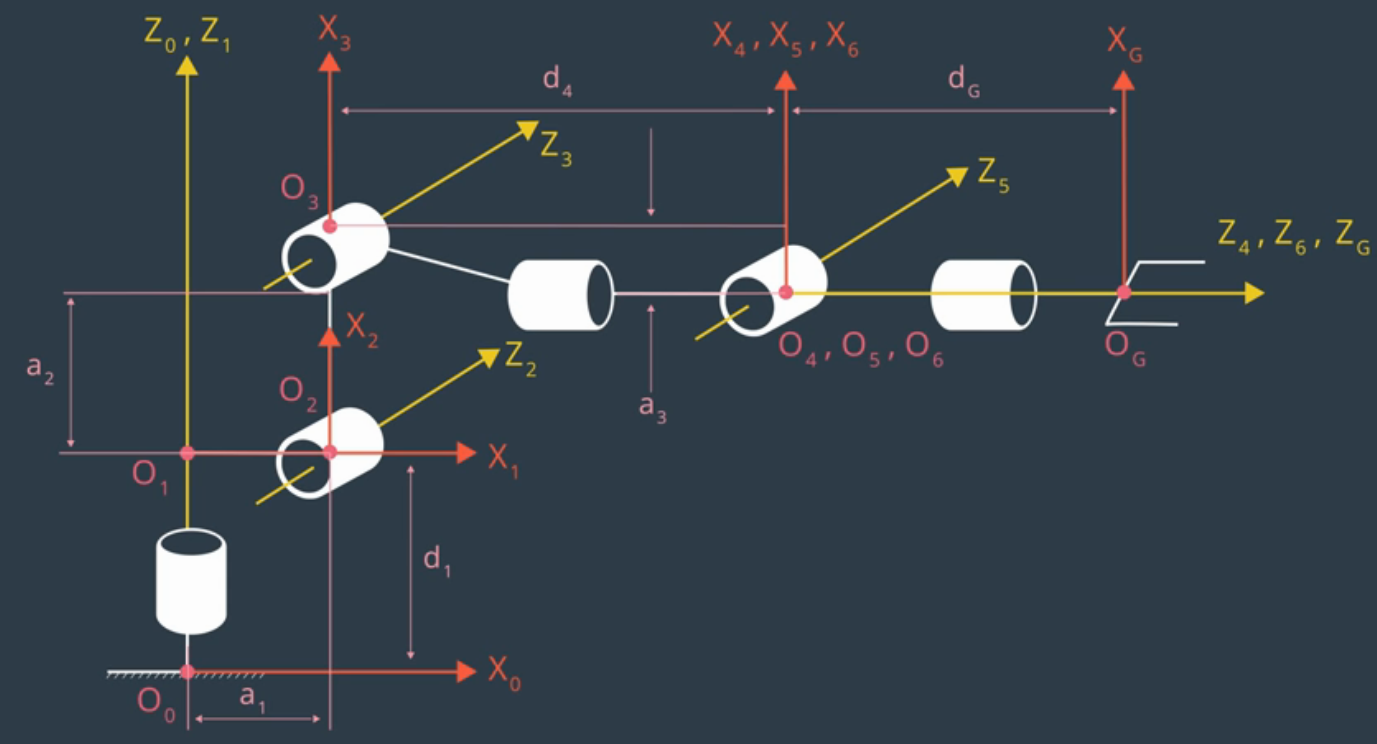
\includegraphics[width=\linewidth]{KR210RF.png}
    \caption{Schematic showing reference frames for each joint as shown in project lesson 10}
    \label{fig:RFscheme}
\end{figure}

Using the reference frames the Denavit-Hartenberg parameters can be defined. For this project the DH parameters are defined using the convention described by John J. Craig in his book Introduction to Robotics: Mechanics and Control. The definitions are as follows (from lesson 2 section 12):

\begin{itemize}
    \item Twist angle ($\alpha _{i-1}$): angle between $\hat{Z}_{i-1}$ and $\hat{Z}_i$ measured about $\hat{X}_{i-1}$ in a right hand sense.
    \item Link length ($a_{i-1}$): distance from $\hat{Z}_{i-1}$ to $\hat{Z}_i$ measured along $\hat{X}_{i-1}$.
    \item Link offset ($d_i$): signed distance from $\hat{X}_{i-1}$ to $\hat{X}_i$ measured along $\hat{Z}_i$.
    \item Joint angle: angle between $\hat{X}_{i-1}$ and $\hat{X}_i$ measured about $\hat{Z}_i$ in a right hand sense.
\end{itemize}

\begin{table}[H]
\centering
\begin{tabular}{|c|c|r|c|c|l|}
    \hline
    i & Transform & $\alpha _{i-1}$ & $a_{i-1}$ & $d_i$ & $\theta _i$ \\ \hline
    1 & $T_1^0$ & 0 & 0 & 0.75 & $\theta _1$ \\ \hline
    2 & $T_2^1$ & $-\frac{\pi}{2}$ & 0.35 & 0 & $\theta _2 - \frac{\pi}{2}$ \\ \hline
    3 & $T_3^2$ & 0 & 1.25 & 0 & $\theta _3$ \\ \hline
    4 & $T_4^3$ & $-\frac{\pi}{2}$ & -0.054 & 1.5 & $\theta _4$ \\ \hline
    5 & $T_5^4$ & $\frac{\pi}{2}$ & 0 & 0 & $\theta _5$ \\ \hline
    6 & $T_6^5$ & $-\frac{\pi}{2}$ & 0 & 0 & $\theta _6$ \\ \hline
    7 & $T_G^6$ & 0 & 0 & 0.303 & 0 \\ \hline

\end{tabular}
\caption{\label{tab:table-name}Denavit-Hartenberg parameter table with values derived from the URDF file}
\end{table}

\subsection{2. Using the DH parameter table you derived earlier, create individual transformation matrices about each joint. In addition, also generate a generalized homogeneous transform between base\_link and gripper\_link using only end-effector(gripper) pose.}

The general form of a homogeneous transform between two reference frames described using our convention can be written as follows:
\[T_{i-1}^i =
\begin{bmatrix}
    \cos(\theta _i) & -\sin(\theta _i) & 0 & a_{i-1} \\
    \sin(\theta _i)\cos(\alpha _{i-1}) & \cos(\theta _i)\cos(\alpha _{i-1}) & -\sin(\alpha _{i-1}) & -\sin(\alpha _{i-1})d_i \\
    \sin(\theta _i)\sin(\alpha _{i-1}) & \cos(\theta _i)\sin(\alpha _{i-1}) & \cos(\alpha _{i-1}) & \cos(\alpha _{i-1})d_i \\
    0 & 0 & 0 & 1

\end{bmatrix}
\]
From this equation the individual transform matrices can be derived.
\[T_{1}^0 =
\begin{bmatrix}
    \cos(\theta _1) & -\sin(\theta _1) & 0 & a_{0} \\
    \sin(\theta _1)\cos(\alpha _{0}) & \cos(\theta _1)\cos(\alpha _{0}) & -\sin(\alpha _{0}) & -\sin(\alpha _{0})d_1 \\
    \sin(\theta _1)\sin(\alpha _{0}) & \cos(\theta _1)\sin(\alpha _{0}) & \cos(\alpha _{0}) & \cos(\alpha _{0})d_1 \\
    0 & 0 & 0 & 1

\end{bmatrix}
\]
\[T_{2}^1 =
\begin{bmatrix}
    \cos(\theta _2) & -\sin(\theta _2) & 0 & a_{1} \\
    \sin(\theta _2)\cos(\alpha _{1}) & \cos(\theta _2)\cos(\alpha _{1}) & -\sin(\alpha _{1}) & -\sin(\alpha _{1})d_2 \\
    \sin(\theta _2)\sin(\alpha _{1}) & \cos(\theta _2)\sin(\alpha _{1}) & \cos(\alpha _{1}) & \cos(\alpha _{1})d_2 \\
    0 & 0 & 0 & 1

\end{bmatrix}
\]
\[T_{3}^2 =
\begin{bmatrix}
    \cos(\theta _3) & -\sin(\theta _3) & 0 & a_{2} \\
    \sin(\theta _3)\cos(\alpha _{2}) & \cos(\theta _3)\cos(\alpha _{2}) & -\sin(\alpha _{2}) & -\sin(\alpha _{2})d_3 \\
    \sin(\theta _3)\sin(\alpha _{2}) & \cos(\theta _3)\sin(\alpha _{2}) & \cos(\alpha _{2}) & \cos(\alpha _{2})d_3 \\
    0 & 0 & 0 & 1

\end{bmatrix}
\]
\[T_{4}^3 =
\begin{bmatrix}
    \cos(\theta _4) & -\sin(\theta _4) & 0 & a_{3} \\
    \sin(\theta _4)\cos(\alpha _{3}) & \cos(\theta _4)\cos(\alpha _{3}) & -\sin(\alpha _{3}) & -\sin(\alpha _{3})d_4 \\
    \sin(\theta _4)\sin(\alpha _{3}) & \cos(\theta _4)\sin(\alpha _{3}) & \cos(\alpha _{3}) & \cos(\alpha _{3})d_4 \\
    0 & 0 & 0 & 1

\end{bmatrix}
\]
\[T_{5}^4 =
\begin{bmatrix}
    \cos(\theta _5) & -\sin(\theta _5) & 0 & a_{4} \\
    \sin(\theta _5)\cos(\alpha _{4}) & \cos(\theta _5)\cos(\alpha _{4}) & -\sin(\alpha _{4}) & -\sin(\alpha _{4})d_5 \\
    \sin(\theta _5)\sin(\alpha _{4}) & \cos(\theta _5)\sin(\alpha _{4}) & \cos(\alpha _{4}) & \cos(\alpha _{4})d_5 \\
    0 & 0 & 0 & 1

\end{bmatrix}
\]
\[T_{6}^5 =
\begin{bmatrix}
    \cos(\theta _6) & -\sin(\theta _6) & 0 & a_{5} \\
    \sin(\theta _6)\cos(\alpha _{5}) & \cos(\theta _6)\cos(\alpha _{5}) & -\sin(\alpha _{5}) & -\sin(\alpha _{5})d_6 \\
    \sin(\theta _6)\sin(\alpha _{5}) & \cos(\theta _6)\sin(\alpha _{5}) & \cos(\alpha _{5}) & \cos(\alpha _{5})d_6 \\
    0 & 0 & 0 & 1

\end{bmatrix}
\]
\[T_{G}^6 = T_7^6 =
\begin{bmatrix}
    \cos(\theta _7) & -\sin(\theta _7) & 0 & a_{6} \\
    \sin(\theta _7)\cos(\alpha _{6}) & \cos(\theta _7)\cos(\alpha _{6}) & -\sin(\alpha _{6}) & -\sin(\alpha _{6})d_7 \\
    \sin(\theta _7)\sin(\alpha _{6}) & \cos(\theta _7)\sin(\alpha _{6}) & \cos(\alpha _{6}) & \cos(\alpha _{6})d_7 \\
    0 & 0 & 0 & 1

\end{bmatrix}
\]

The total homogeneous transform between the base link and the end link can be found by multiplying the individual transforms together
\[T_G^0 = T_1^0 * T_2^1 * T_3^2 * T_4^3 * T_5^4 * T_6^5 * T_G^6 \]

Because of the difference in the way the orientation of the DH frames are defined versus the way the URDF file is written, two additional rotations must be applied to the gripper frame: a 180 degree rotation about the z-axis, followed by a -90 degree rotation about the y-axis.

\[R_z = 
\begin{bmatrix}
    \cos(\pi) & -\sin(\pi) & 0 & 0 \\
    \sin(\pi) & \cos(\pi) & 0 & 0 \\
    0 & 0 & 1 & 0 \\
    0 & 0 & 0 & 1
\end{bmatrix}
\]

\[R_y = 
\begin{bmatrix}
    \cos(-\frac{\pi}{2}) & 0 & \sin(-\frac{\pi}{2}) & 0 \\
    0 & 1 & 0 & 0 \\
    -\sin(-\frac{\pi}{2}) & 0 & \cos(-\frac{\pi}{2}) & 0 \\
   0 & 0 & 0 & 1
\end{bmatrix}
\]

The total transform can then be described as:
\[T_{total} = T_G^0 * R_z * R_y \]


\subsection{3. Decouple Inverse Kinematics problem into Inverse Position Kinematics and inverse Orientation Kinematics; doing so derive the equations to calculate all individual joint angles.}
Because the axes of joints 4, 5, and 6 intersect at a single point, the position and orientation of the end effector are kinematically decoupled. Joints 4, 5, and 6 form a spherical wrist that determine the orientation of the end effector, while joints 1, 2 and 3 determine the location of the end effector.

\subsubsection{Inverse Position}

\paragraph{Wrist Center Position}

The first step for finding the first three joint angles is to use the end effector position that is passed to the inverse kinematics server to find the location of the wrist center. Because the wrist center is located at joint five, it can be found by starting at the end effector location and subtracting the link length from joint five to joint 6 and from joint 6 to the end effector along the $Z_G$ axis as shown in figure \ref{fig:RFscheme}.
This can be written mathematically as follows:

\[
\begin{bmatrix}
    w_x \\
    w_y \\
    w_z
\end{bmatrix}
=
\begin{bmatrix}
    p_x \\
    p_y \\
    p_z
\end{bmatrix}
-
\begin{bmatrix}
    d_6 + d_7 \\
    d_6 + d_7 \\
    d_6 + d_7
\end{bmatrix}
*
\begin{bmatrix}
    n_x \\
    n_y \\
    n_z \\
\end{bmatrix}    
\]
Where:
\begin{itemize}
    \item w = wrist center location
    \item p = end effector location
    \item n = the vector along the $Z_G$ axis
\end{itemize}

\paragraph{Joint 1 - $\theta _1$}
\begin{figure}[H]
    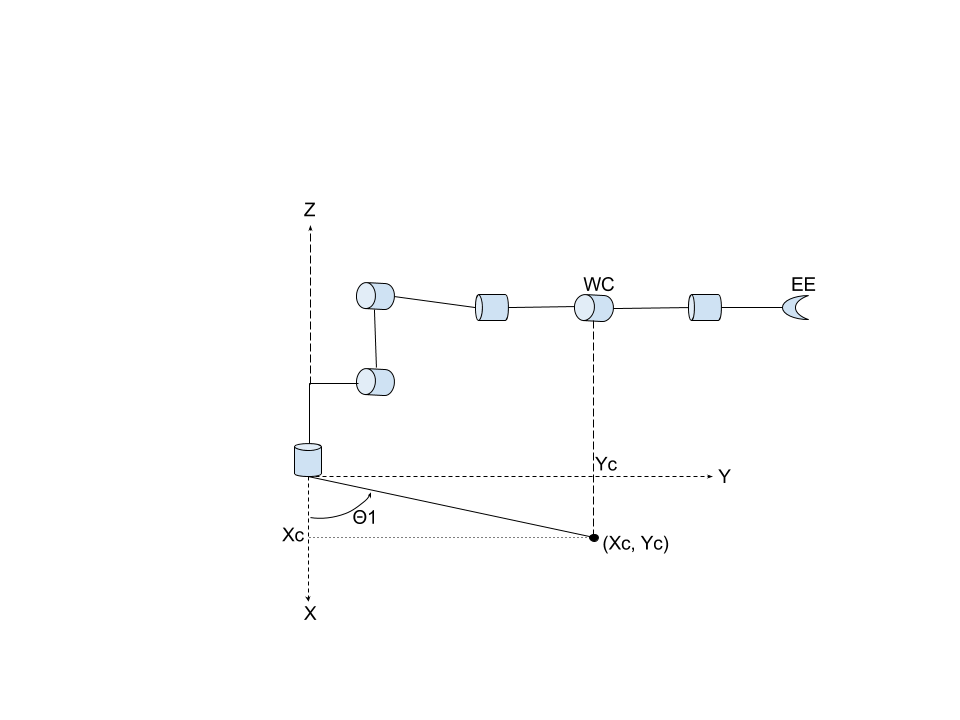
\includegraphics[width=\linewidth]{theta1.png}
    \caption{Diagram for calculating theta 1.}
    \label{fig:theta3}
\end{figure}
\begin{itemize}
    \item EE = end effector
    \item WC = wrist center
    \item $X_c$ = X component of wrist center position
    \item $Y_c$ = Y component of wrist center position
\end{itemize}
Once the wrist center location is known, $\theta _1$ can be found by using the projection of the wrist center onto the XY plane. $\theta _1$ is the arctangent of the X and Y components of the wrist center position.
\[\theta _1 = atan2(Y_c, X_c)\]

\paragraph{Joint 2 - $\theta _2$}
\begin{figure}[H]
    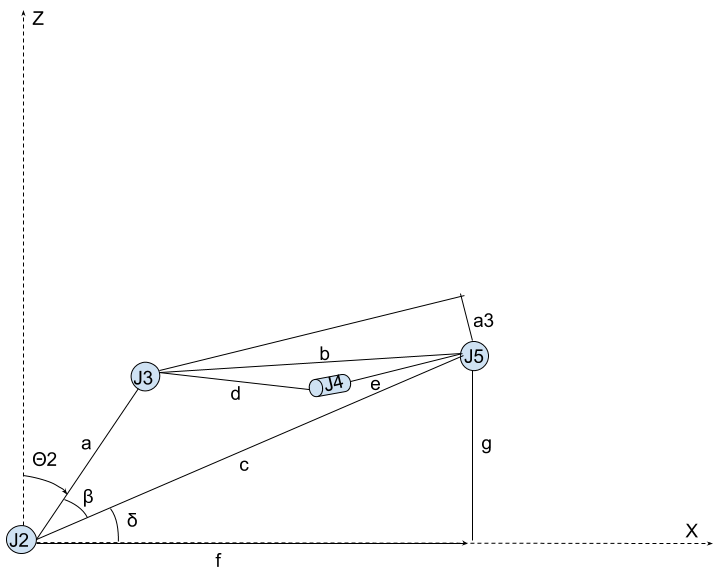
\includegraphics[width=\linewidth]{theta2.png}
    \caption{Diagram for calculating theta 2.}
    \label{fig:theta3}
\end{figure}
\begin{figure}[H]
    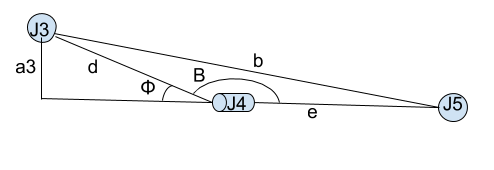
\includegraphics[width=\linewidth]{offsetangle.png}
    \caption{Diagram for calculating the length of $b$.}
    \label{fig:offsetangle}
\end{figure}
\begin{itemize}
    \item $a$ = link length from joint 2 to joint 3
    \item $b$ = straight line distance between joint 3 and joint 5
    \item $c$ = straight line distance between joint 2 and joint 5
    \item $d$ = link length from joint 3 to joint 4
    \item $e$ = link length from joint 4 to joint 5
    \item $f$ = the projection of c onto the XY plane
    \item $g$ = the distance between the Z position of joint 5 and the Z position of joint 2
    \item $a3$ = the vertical offset between joint 3 and joint 4
    \item $\beta$ = the angle between $a$ and $c$
    \item $\delta$ = the angle between $c$ and $f$
    \item $B$ = the angle between $d$ and $e$
    \item $\phi$ = the offset angle caused by a3
\end{itemize}

$a, d, e,$ and $a3$ are all from the DH parameter table. \\
Using figure \ref{fig:offsetangle}, b can be calculated as follows:
\[\phi = asin\bigg(\frac{a3}{d}\bigg)\]
\[B = \pi - \phi\]
\[b = \sqrt{d^2 + e^2 -2de\cos(B)}\]
Since the position of J5 is known after finding the wrist center and the position of J2 can be calculated using the DH parameter table and rotating by $\theta _1$, c can be found by taking the distance between the two points:
\[c = \sqrt{(J5_x - J2_x)^2 + (J5_y - J2_y)^2 + (J5_z - J2_z)^2}\]
$f$ can be found by removing the Z term from the $c$ equation:
\[f = \sqrt{(J5_x - J2_x)^2 + (J5_y - J2_y)^2}\]
$g$ is simply the distance between two points on the Z axis:
\[g = J5_z - J2_z\]
$\beta$ can be found using the law of cosines because the lengths of all three sides of the triangle $abc$ are known:
\[\beta = acos\bigg(\frac{b^2 - a^2 - c^2}{-2ac}\bigg)\]
since $g$ and $f$ are known, $\delta$ can be found using the arctangent:
\[\delta = atan2(g,f)\]
because the sum of $\theta _2$, $\beta$ and $\delta$ forms a right angle, $\theta _2$ can be written as:
\[\theta _2 = \frac{\pi}{2} - \beta - \delta\]

\paragraph{Joint 3 - $\theta _3$}
\begin{figure}[H]
    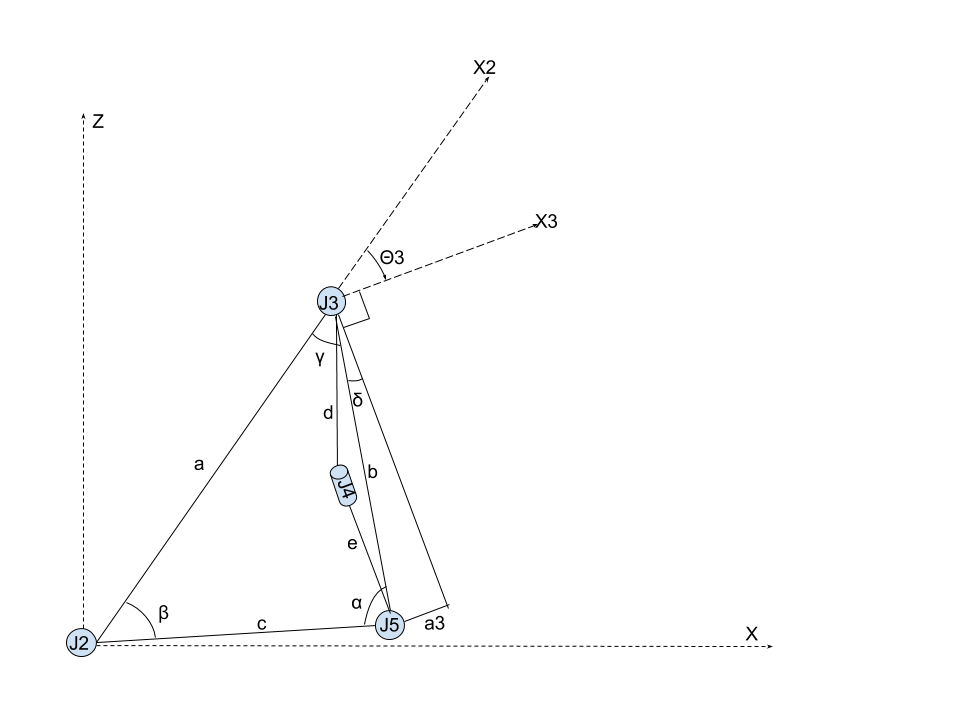
\includegraphics[width=\linewidth]{theta3.png}
    \caption{Diagram for calculating theta 3.}
    \label{fig:theta3}
\end{figure}
\begin{itemize}
    \item $a$ = link length from joint 2 to joint 3
    \item $b$ = straight line distance between joint 3 and joint 5
    \item $c$ = straight line distance between joint 2 and joint 5
    \item $d$ = link length from joint 3 to joint 4
    \item $e$ = link length from joint 4 to joint 5
    \item $a3$ = the vertical offset between joint 3 and joint 4
    \item $\alpha$ = the angle between $b$ and $c$
    \item $\beta$ = the angle between $a$ and $c$
    \item $\gamma$ = the angle between $a$ and $b$
    \item $\delta$ = the angle between $b$ and the Y axis of joint 3
\end{itemize}
$a, d, e,$ and $a3$ are all from the DH parameter table. \\
$b$ and $c$ are calculated the same way as in the $\theta _2$ calculation. \\
Because all side lengths of the triangle $abc$ are known, $\gamma$ can be found using the law of cosines:
\[\gamma = acos\bigg(\frac{c^2 - a^2 - b^2}{-2ab}\bigg)\]
\[\delta = asin\bigg(\frac{a3}{b}\bigg)\]
\[\theta _3 = \frac{\pi}{2} - \delta - \gamma\]

\subsubsection{Inverse Orientation}

\paragraph{Joint 4 - $\theta _4$}

\paragraph{Joint 5 - $\theta _5$}

\paragraph{Joint 6 - $\theta _6$}

\section{Project Implementation}

\subsubsection{1. Fill in the `IK\_server.py` file with properly commented python code for calculating Inverse Kinematics based on previously performed Kinematic Analysis. Your code must guide the robot to successfully complete 8/10 pick and place cycles. Briefly discuss the code you implemented and your results.}


Here I'll talk about the code, what techniques I used, what worked and why, where the implementation might fail and how I might improve it if I were going to pursue this project further.  


And just for fun, another example image:
% ![alt text][image3]

\end{document}
